
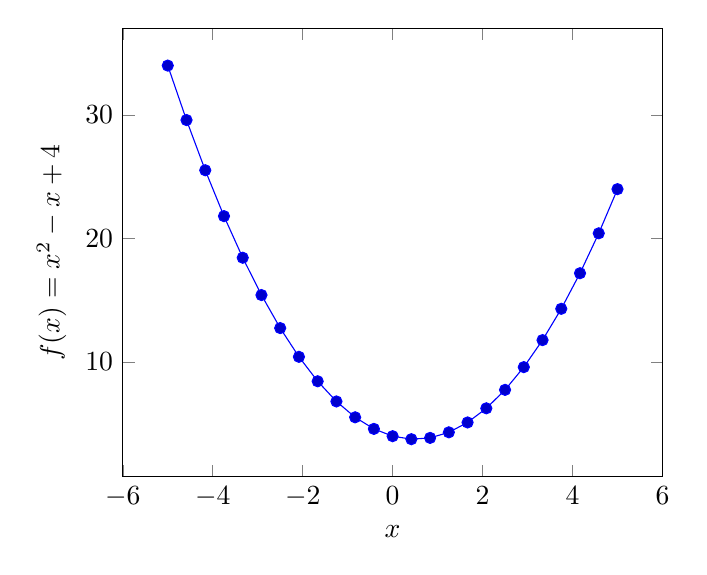
\begin{tikzpicture}
  \begin{axis}[ 
    xlabel=$x$,
    ylabel={$f(x) = x^2 - x +4$}
  ] 
    \addplot {x^2 - x +4}; 
  \end{axis}
\end{tikzpicture}

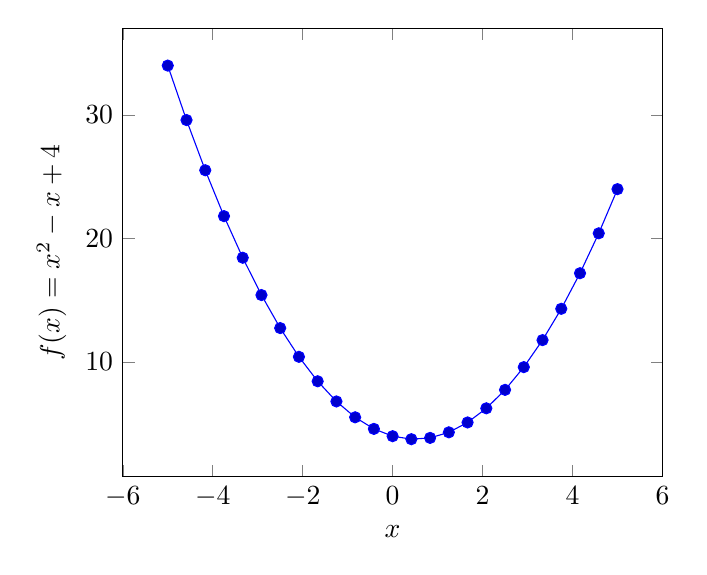
\begin{tikzpicture}
  \begin{axis}[ 
    xlabel=$x$,
    ylabel={$f(x) = x^2 - x +4$}
  ] 
    \addplot {x^2 - x +4}; 
  \end{axis}
\end{tikzpicture}

\begin{tikzpicture}
\datavisualization [school book axes,
                    visualize as smooth line,
                    y axis={label={$y=x^2$}},
                    x axis={label} ]

data [format=function] {
      var x : interval [0:1] samples 7;
      func y = \value x*\value x;
      };
\end{tikzpicture}

